\documentclass[conference]{IEEEtran}
\IEEEoverridecommandlockouts
\usepackage{cite}
\usepackage{amsmath,amssymb,amsfonts}
\usepackage{graphicx}
\usepackage{booktabs}
\usepackage{multirow}
\usepackage{url}
\usepackage{xcolor}
\usepackage{tikz}
\usetikzlibrary{arrows.meta,positioning,fit,backgrounds}
\usepackage[hidelinks]{hyperref}

\newcommand{\cqlppo}{CQL$\to$PPO}
\newcommand{\bcppo}{BC$\to$PPO}

\begin{document}

\title{What Does a Frame of Delay Buy? Learned Per-Frame QP Control for x265 and x264, and Where Reinforcement Learning Helps}

\author{\IEEEauthorblockN{[Author Name]}
\IEEEauthorblockA{EE599 Course Project\\
University of Southern California, Los Angeles, CA, USA}}

\maketitle

\begin{abstract}
Rate control decides how many bits each frame of a video receives. An offline search that sees a whole group of pictures (GOP) in advance and tries hundreds of quantization-parameter (QP) plans with real encodes saves about 10\% of the bits that the encoder's own constant-QP mode needs for the same PSNR, while the encoders' built-in single-pass and two-pass rate controllers fall short of constant QP on the same budgets. The search cannot run in a live encoder. We ask how much of its gain a policy that encodes each frame once can recover, and how this share changes with the number of future frames the policy may inspect (the lookahead $k$), from strictly causal ($k{=}0$) to the full GOP ($k{=}29$). On 2{,}061 GOPs from 189 sources, encoded with real x265 (HEVC) and x264 (AVC), we train and compare imitation learning, offline reinforcement learning (CQL, IQL), online RL (PPO, A2C, DQN), budget-constrained RL (Lagrangian and PID-Lagrangian), model-predictive control, ensembles and gated lookahead. A single-pass policy recovers about half of the search's bit saving; nearly all of the benefit of lookahead is reached with 2--3 frames, and longer windows do not help. Within one GOP, imitation of the search already obtains most of the saving, and RL's distinct contribution is budget reliability: Lagrangian RL raises the score over imitation by +2.7 (x265) and +3.7 (x264) points at $k{=}0$ and cuts the share of over-budget GOPs from 17--19\% to 1--2\%. When eight GOPs share one budget whose matching QP is unknown, imitation of the hindsight plan fails ($-17$ to $-20$ points) while PPO beats the best constant QP chosen in hindsight by +3.2 (x265) and +1.9 (x264) points at 1\% over-budget rate. We report all results with seed-level and bootstrap confidence intervals, document negative results (MPC, DQN, A2C), and release the experimental design for reproduction.
\end{abstract}

\begin{IEEEkeywords}
video coding, rate control, HEVC, H.264/AVC, x265, x264, reinforcement learning, offline RL, constrained RL, lookahead
\end{IEEEkeywords}

%=====================================================================
\section{Introduction}
%=====================================================================
Every video encoder must answer one question many times per second: which quantization parameter (QP) should the next frame use? A lower QP spends more bits for higher fidelity; a higher QP saves bits at a cost in quality. The \emph{rate controller} chooses QPs so that the stream meets a bit budget while preserving as much quality as possible. Because frames are predicted from one another, the choice is a sequential decision problem: bits spent on an I frame or on early P frames improve the references of every later frame, and a scene cut makes the next frames expensive regardless of what came before~\cite{sullivan1998rdo,ortega1998rd}.

Production encoders solve this with hand-designed models and, when latency allows, with a lookahead buffer: x264 and x265 analyse upcoming frames with a fast first pass and propagate their importance backwards (MB-tree / CU-tree)~\cite{garrett2009mbtree,x264,x265}. Lookahead, however, costs delay and memory. A live encoder designer must decide how many frames of delay to pay for, and today this decision is made by experience rather than by measurement.

This paper measures it. We first establish a ceiling: an offline \emph{hindsight search} that sees a whole 30-frame GOP and evaluates hundreds of per-frame QP plans with real encodes. It saves $\sim$10\% of the bits that the encoder's own constant-QP mode needs at equal PSNR, on budgets where the encoders' built-in rate control is \emph{worse} than constant QP. The search needs 300--600 trial encodes per GOP and cannot run live. We then train single-pass policies that see $k$ future frames and ask: \emph{what share of the search's gain can a policy capture in one encode, and how does that share change as $k$ grows from 0 (strictly causal) to the full GOP?}

Reinforcement learning (RL) is the natural tool, and the second question of this work is whether it actually earns its place. We compare imitation of the search, offline RL, online RL, budget-constrained RL, model-predictive control and several extensions under identical data and evaluation, on two encoders. We find that the answer depends on what the policy must learn. Within a single GOP, the search is a near-perfect teacher, and imitating it obtains most of the saving; RL's contribution is to make the policy hold its budget. When several GOPs share one budget, the search's plan relies on information a causal controller lacks, imitation breaks down, and RL becomes essential.

\textbf{Contributions.}
\begin{itemize}
\item A reproducible testbed of 2{,}061 GOPs from 189 sources with real x265 and x264 encodes, per-frame QP control, and a hindsight-search ceiling (Section~\ref{sec:setup}).
\item The lookahead curve: the share of the search's gain captured by a single-pass policy for $k \in \{0,\dots,10,15,20,29\}$ on both encoders. Two to three frames of lookahead capture essentially all of the available benefit (Section~\ref{sec:lookahead}).
\item A controlled comparison of eleven learning approaches, showing where RL helps: constrained RL turns an imitation policy into a budget-reliable one, and a plain RL policy controlling a multi-GOP stream beats the best constant QP chosen in hindsight while imitation fails (Sections~\ref{sec:methods}--\ref{sec:multigop}).
\item Negative and corrective findings, including model exploitation by MPC and by model-based pre-training, and a metric artefact of averaging PSNR across GOPs (Section~\ref{sec:discussion}).
\end{itemize}

%=====================================================================
\section{Motivation}
%=====================================================================
\textbf{Why per-frame QP matters.} In a hybrid video coder the distortion of frame $t$ depends on its own QP and on the quality of its references. Allocating more bits to frames that many later frames reference (the I frame, the first P frames of a scene) lowers the total cost of the GOP. Constant QP ignores this structure, and the encoders' adaptive tools (adaptive quantization, MB-tree/CU-tree) approximate it from a lookahead analysis~\cite{garrett2009mbtree}.

\textbf{Why lookahead has a price.} Every frame of lookahead adds one frame period of encoding delay and one frame of buffer memory. In low-latency streaming, video conferencing, cloud gaming and broadcast contribution, the delay budget is a few frames. Knowing how much quality each extra frame buys turns this into an engineering trade-off rather than a guess.

\textbf{Why learning.} The search shows what is achievable with perfect information, but it is a planning procedure, not a controller. A learned policy can amortize the search into a function that maps the encoder's state and the visible lookahead to a QP in microseconds. Whether it should be learned by imitation or by RL, and with which algorithm, is not obvious: imitation is simple and data-efficient but inherits the teacher's assumption of full information; RL optimizes the true objective under the policy's own information but needs many episodes, and every episode here costs real encodes.

\textbf{Why budgets are hard.} A rate controller is judged on two things at once: quality at a given rate, and staying within the budget. A controller that saves bits on average but overshoots its budget on one GOP in five is not deployable. Our metric therefore penalizes overshoot explicitly, and we report the share of over-budget GOPs alongside every score.

%=====================================================================
\section{Background}
%=====================================================================
\subsection{Video coding and rate control}
H.264/AVC~\cite{wiegand2003h264} and HEVC~\cite{sullivan2012hevc} are block-based hybrid coders: each block is predicted (intra or from reference frames), and the residual is transformed and quantized. The quantization step size doubles every 6 QP units, so bits fall roughly exponentially and PSNR roughly linearly in QP. Encoders select coding modes by rate--distortion optimization (RDO), minimizing $D + \lambda R$ with a Lagrange multiplier $\lambda$ tied to QP~\cite{sullivan1998rdo,ortega1998rd}.

Rate control maps a target bit rate to QPs. Classical approaches model rate as a function of QP or of $\lambda$ and correct the model with feedback~\cite{chen2007rcsurvey}; HEVC's reference software uses $R$--$\lambda$ models~\cite{li2014lambda}. The open-source encoders x264~\cite{x264} and x265~\cite{x265} offer constant QP (CQP), constant rate factor (CRF), single-pass average bit rate (ABR), two-pass ABR, and a VBV buffer constraint. Their quality comes largely from adaptive quantization (AQ) and from MB-tree/CU-tree, which estimates from a lookahead how much each block is referenced and lowers its QP accordingly~\cite{garrett2009mbtree}.

Compression efficiency is usually compared at equal quality: the Bj{\o}ntegaard delta rate (BD-rate) integrates the bit-rate difference between two rate--distortion curves~\cite{bjontegaard2001}. Our score uses the same idea at a single operating point (Section~\ref{sec:problem}).

\subsection{Reinforcement learning}
A Markov decision process (MDP) is a tuple $(\mathcal{S},\mathcal{A},P,r,\gamma)$. A policy $\pi(a\mid s)$ induces a return $G = \sum_t \gamma^t r_t$; RL seeks $\pi^\star = \arg\max_\pi \mathbb{E}_\pi[G]$~\cite{sutton2018rl}. The action-value function $Q^\pi(s,a)$ is the expected return after taking $a$ in $s$; the value $V^\pi(s) = \mathbb{E}_{a\sim\pi}Q^\pi(s,a)$; the advantage $A^\pi = Q^\pi - V^\pi$.

\textbf{Policy gradient and actor--critic.} The policy-gradient theorem gives $\nabla_\theta J = \mathbb{E}[\nabla_\theta \log \pi_\theta(a\mid s)\, A^\pi(s,a)]$~\cite{williams1992reinforce,sutton2018rl}. Actor--critic methods learn $V$ as a baseline~\cite{konda2000actorcritic}. \emph{A2C} is the synchronous variant of A3C~\cite{mnih2016a3c}, taking one gradient step per short rollout. \emph{PPO}~\cite{schulman2017ppo} reuses each rollout for several epochs and keeps the update close to the data-collecting policy with the clipped surrogate
\begin{equation}
L^{\text{clip}}(\theta)=\mathbb{E}_t\!\left[\min\!\big(\rho_t \hat A_t,\ \operatorname{clip}(\rho_t,1{-}\epsilon,1{+}\epsilon)\hat A_t\big)\right],
\end{equation}
where $\rho_t = \pi_\theta(a_t\mid s_t)/\pi_{\theta_{\text{old}}}(a_t\mid s_t)$ and $\hat A_t$ is estimated with GAE~\cite{schulman2016gae}.

\textbf{Value-based RL.} \emph{DQN}~\cite{mnih2015dqn} learns $Q$ by minimizing the temporal-difference error $\big(r + \gamma \max_{a'} Q_{\bar\theta}(s',a') - Q_\theta(s,a)\big)^2$ with a replay buffer and a target network $\bar\theta$, acting $\epsilon$-greedily.

\textbf{Imitation and offline RL.} \emph{Behaviour cloning} (BC) fits $\pi(a\mid s)$ to expert state--action pairs by maximum likelihood~\cite{pomerleau1989alvinn}; it suffers from compounding errors when the learner's states drift from the expert's~\cite{ross2011dagger}. \emph{Offline RL} learns from a fixed dataset without interaction~\cite{levine2020offline}. Its central difficulty is overestimating actions absent from the data. \emph{CQL}~\cite{kumar2020cql} adds a regularizer $\alpha\,\mathbb{E}_s[\log\sum_a e^{Q(s,a)} - Q(s,a_{\text{data}})]$ that pushes down the values of unseen actions. \emph{IQL}~\cite{kostrikov2022iql} avoids querying unseen actions altogether: it fits $V$ by expectile regression on $Q$ and extracts a policy by advantage-weighted regression.

\textbf{Constrained RL.} A constrained MDP~\cite{altman1999cmdp} maximizes reward subject to $\mathbb{E}[c] \le d$. The Lagrangian relaxation maximizes $r - \lambda c$; $\lambda$ can be fixed, updated by gradient ascent on the constraint violation~\cite{tessler2019rcpo}, or driven by a PID controller to reduce oscillation~\cite{stooke2020pid}.

\textbf{Model-based control.} With a learned dynamics model, model-predictive control (MPC) re-plans at every step, for example with the cross-entropy method (CEM)~\cite{rubinstein1997cem,chua2018pets}. Alternatively, a policy can be trained on model rollouts (Dyna~\cite{sutton1991dyna}, MBPO~\cite{janner2019mbpo}); both are vulnerable to the controller exploiting model errors~\cite{janner2019mbpo}. \emph{Deep ensembles} average independently trained networks to reduce variance~\cite{lakshminarayanan2017ensembles}.

\subsection{Learning-based rate control}
RL has been applied to HEVC intra-frame rate control~\cite{hu2018rlintra}, and MuZero~\cite{schrittwieser2020muzero} with self-competition was deployed for rate control in VP9, where the agent sets frame QPs over a whole video under a bit-rate constraint~\cite{mandhane2022muzero}. These works optimize a fixed information setting. Our focus is the dependence of the attainable gain on lookahead, and a controlled comparison of learning paradigms against a measured hindsight ceiling on two production encoders.

%=====================================================================
\section{Problem Formulation}\label{sec:problem}
%=====================================================================
\subsection{Episode, action, and budget}
An episode is one GOP of 30 frames (an IDR frame followed by 29 P frames, no B frames) at $320{\times}180$, coded with x265 or x264 at a fixed preset with AQ and MB/CU-tree disabled, so that each frame obeys its QP exactly. The budget is the number of bits the encoder's own constant-QP mode spends on the GOP at base QP $b \in \{30, 38\}$ (two operating points per GOP). Frame $t$ is coded at
\begin{equation}
q_t = b + s_t + a_t,\qquad a_t \in \{-3,\dots,+3\},
\end{equation}
where $s_t$ is a fixed spend-early pattern (STATIC: $-6$ for the I frame, $-3$ for P frames 1--9, $+3$ for P frames 10--29) and $a_t$ is the controller's action. The controller acts after observing frames $0..t{-}1$ encoded, their bits, and the features of frames $t..t{+}k$.

\subsection{Score}
Let $C(\cdot)$ be the GOP's constant-QP curve (bits as a function of PSNR, interpolated in log-bits over QP 18--50). For an encode with $B$ bits and mean PSNR $P$ under budget $\bar B$,
\begin{align}
\text{saving} &= 100\,\big(1 - B / C(P)\big),\\
\text{over} &= 100\,\max(0,\ B/\bar B - 1),\\
\text{score} &= \text{saving} - 2\cdot\text{over}.
\end{align}
Saving is the percentage of bits saved at equal PSNR relative to the encoder's own constant QP (a single-point BD-rate); every 1\% of overshoot costs 2 points. Constant QP at $b$ scores 0 by construction. PSNR is the 6:1:1-weighted YUV PSNR of the decoded frames against the source, averaged over frames.

\subsection{Hindsight search (the ceiling)}
For every (GOP, budget) pair, a hill-climbing search starts from STATIC and proposes local moves on the 30 offsets (single-frame $\pm1$, runs of 2--6 frames, bit transfers between frames), keeping a move when the score does not decrease. Every proposal is a real encode; we run two seeds of 300 encodes. All evaluated plans are logged and form the offline-learning dataset. The best plan's score is the ceiling.

\subsection{Research question and the measured share}
For a single-pass policy $\pi_k$ with lookahead $k$, we report its score and saving and the \emph{share of the search's gain} it captures, $\text{share}_k = \overline{\text{saving}}(\pi_k)/\overline{\text{saving}}(\text{search})$ (and the same ratio for the score), averaged over test cases, for $k \in \{0,1,\dots,10,15,20,29\}$.

%=====================================================================
\section{Methods}\label{sec:approach}
%=====================================================================
\begin{figure}[t]
\centering
\resizebox{\columnwidth}{!}{%
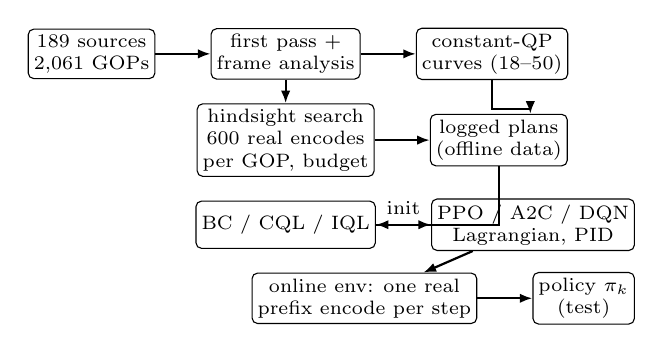
\begin{tikzpicture}[font=\scriptsize, node distance=3mm and 7mm,
  box/.style={draw, rounded corners=2pt, align=center, minimum height=6mm, inner sep=2pt, fill=white},
  arr/.style={-{Latex[length=1.6mm]}, thick}]
\node[box] (src) {189 sources\\2{,}061 GOPs};
\node[box, right=of src] (fp) {first pass +\\frame analysis};
\node[box, right=of fp] (cqp) {constant-QP\\curves (18--50)};
\node[box, below=of fp] (search) {hindsight search\\600 real encodes\\per GOP, budget};
\node[box, right=of search] (data) {logged plans\\(offline data)};
\node[box, below=of search] (off) {BC / CQL / IQL};
\node[box, right=of off] (rl) {PPO / A2C / DQN\\Lagrangian, PID};
\node[box, below=of off, xshift=10mm] (env) {online env: one real\\prefix encode per step};
\node[box, right=of env] (pol) {policy $\pi_k$\\(test)};
\draw[arr] (src) -- (fp); \draw[arr] (fp) -- (cqp);
\draw[arr] (fp) -- (search); \draw[arr] (search) -- (data);
\draw[arr] (data) |- (off); \draw[arr] (off) -- node[above]{init} (rl);
\draw[arr] (rl) -- (env); \draw[arr] (env) -- (pol);
\draw[arr] (cqp) -- ++(0,-7mm) -| ([xshift=4mm]data.north);
\end{tikzpicture}}
\caption{Pipeline. A first pass and frame analysis give the causal features; constant-QP encodes give the scoring curves and budgets; the hindsight search provides the ceiling and the offline data; learners start offline and are fine-tuned online with real encodes.}
\label{fig:pipeline}
\end{figure}

\subsection{Observation}
The observation has 16 global features and 11 features for each of 30 frame slots (346 values). Global features: position in the GOP, frames remaining, budget level, fraction of the budget spent, remaining budget per remaining frame relative to nominal, last frame's bits and action, last and cumulative ratio of actual to first-pass bits, budget relative to the I frame's cost, scene state (frames since the last cut, distance to the next \emph{visible} cut, share of the visible window's cost before that cut, window mean cost), the visible lookahead length, and an optional scene prior. Per-frame features: first-pass cost relative to the per-frame budget (from one ultrafast encode at QP 30), spatial detail, motion (mean absolute difference), SAD, histogram difference, cut/flash/fade flags, I-frame flag, STATIC offset, and a same-scene flag. Slot 0 is the current frame and slots $1..k$ the lookahead; all features of frames beyond the window are zeroed, and every summary is computed over visible frames only, so the lookahead is strict. Besides fixed $k$ we test scene-aware modes: truncate at the next cut, extend to include it, and look ahead only when a cut is near.

\subsection{Environment and reward}
Each step encodes the prefix of frames $0..t$ with the chosen QPs (we verified that frame bits of a prefix equal those of the full encode), returns real per-frame bits, and at $t{=}29$ decodes for PSNR. The reward is 0 until the end, then $(\text{score} - \text{score}_{\text{STATIC}})/10$ with $\gamma{=}1$. An episode therefore costs 30 real encodes; 60k environment steps are 2{,}000 episodes.

\subsection{Learners}
All learners share the observation, the 7-way action and $256{\times}256$ ReLU networks; Table~\ref{tab:hparams} lists the settings.
\begin{itemize}
\item \textbf{Hand rules:} STATIC; a causal feedback rule that steers cumulative spend to the average STATIC spend curve; a \emph{lookahead rule} that allocates the remaining budget over the visible window in proportion to first-pass cost; and a scene rule adding bits at detected cuts.
\item \textbf{Imitation and offline RL:} BC on the best search plans; CQL and IQL on all logged plans (up to 48 per GOP and budget: the 24 best and 24 random).
\item \textbf{Offline$\to$online:} the offline policy (CQL, or BC) is distilled into the PPO actor (temperature 0.3, value head from $Q$), then fine-tuned with PPO on real encodes (\cqlppo, our core recipe; \bcppo).
\item \textbf{Online from scratch:} PPO, A2C, DQN with the same 60k steps.
\item \textbf{Constrained RL:} \cqlppo{} with reward $(\text{saving} - \lambda\,\text{over})$, fixed $\lambda{=}4$ (Lagrangian), or $\lambda$ driven by a PID controller targeting 5\% of GOPs over budget.
\item \textbf{MPC:} an MLP predicting per-frame bits and PSNR from frame features and QPs, trained on the logged search encodes, calibrated online; CEM re-plans the visible window each frame against a margin-scaled budget chosen on validation.
\item \textbf{Extensions:} warm-started A2C and DQN (CQL initialization); a 3-seed ensemble (mean action probabilities); a per-frame gate choosing between the $k{=}0$ and $k{=}5$ policies with a cost per lookahead frame; extra feedback (achieved PSNR, bit-prediction error) and window-summary features; and Lagrangian/PID fine-tuning of the finished \cqlppo{} policy; one network trained for any $k$ (any-$k$).
\end{itemize}

\begin{table}[t]
\centering\footnotesize
\caption{Training settings (per-GOP setting).}
\label{tab:hparams}
\setlength{\tabcolsep}{3pt}
\begin{tabular}{@{}ll@{}}
\toprule
PPO & 60k env steps, 14 envs, rollout 64, batch 128,\\
 & 5 epochs, ent.\ 0.01, GAE 0.95, lr $10^{-4}$ (fine-tune)\\
 & or $3{\cdot}10^{-4}$ (scratch)\\
A2C / DQN & 60k steps; DQN 1 gradient step per transition, lr $10^{-4}$\\
BC / CQL / IQL & 20k / 50k / 50k steps; CQL $\alpha{=}1$;\\
 & IQL expectile 0.8, $\beta{=}3$\\
Lagrangian / PID & $\lambda{=}4$ / target 5\% over, gains (2, 0.2, 0)\\
Fine-tuning & 40k steps, lr $10^{-4}$, cut GOPs sampled $4\times$\\
Seeds & 3 per configuration\\
\bottomrule
\end{tabular}
\end{table}

\subsection{Multi-GOP setting}\label{sec:mgdef}
To test RL where imitation has no reliable teacher, we build streams of 8 IDR GOPs, either time-ordered GOPs of one source or GOPs of 8 different sources, under one budget $\bar B = s\cdot\sum_g C_g(q_0)$, with $q_0 \in \{30,38\}$ and $s \in \{0.85, 1.0, 1.18\}$ at test (training: $q_0 \in [24,44]$, $s \sim U(0.8,1.25)$). The QP that meets the budget is therefore unknown. At each GOP the controller chooses that GOP's constant QP as an offset $-6..+6$ on a causal \emph{model QP}: the QP at which a first-pass rate model, bits $= c\cdot F\cdot 2^{-(q-30)/5.5}$ (slope fitted on training GOPs, $c$ calibrated online), spends the remaining budget over the remaining GOPs. Offset 0 everywhere is the hand rule. A GOP's bits and PSNR are read from its real constant-QP encodes, so no new encodes are needed and training can use 2M steps. Stream quality is PSNR pooled over MSE, and the score is the saving at equal pooled PSNR against the stream's constant-QP curve minus $2\times$ overshoot. Baselines are the best single constant QP chosen in hindsight (score 0) and a hindsight per-GOP plan (Lagrangian sweep plus greedy refinement over all GOPs' curves). Learners: BC on the hindsight plan, PPO from scratch, and \bcppo, with lookahead $L \in \{0, 2\}$ GOPs.

%=====================================================================
\section{Experimental Setup}\label{sec:setup}
%=====================================================================
\textbf{Data.} 189 sources: YouTube UGC clips~\cite{wang2019ugc}, Xiph test sequences in CIF and HD~\cite{xiph}, and four Blender open movies~\cite{blender}, scaled to $320{\times}180$. Clips contribute evenly spaced, non-overlapping 30-frame windows (8 per Xiph/UGC clip, 90 per long film). We add spliced GOPs built from 2--3 clips of the same split, which contain real scene cuts. Splits are by source (each film is in one split): 1{,}196 train, 386 validation and 479 test GOPs (Table~\ref{tab:data}). With two budgets, the test set has 958 cases.

\begin{table}[t]
\centering\footnotesize
\caption{GOPs per split and family (split by source).}
\label{tab:data}
\begin{tabular}{@{}lrrr@{}}
\toprule
Family & Train & Val & Test\\
\midrule
YouTube UGC & 569 & 168 & 224\\
Xiph CIF & 184 & 24 & 32\\
Xiph HD & 143 & 64 & 32\\
Films (Blender) & 180 & 90 & 131\\
Spliced (2--3 clips) & 120 & 40 & 60\\
\midrule
Total & 1{,}196 & 386 & 479\\
\bottomrule
\end{tabular}
\end{table}

\textbf{Encoders.} x265 4.1 (HEVC) and x264 0.165.3223 (AVC), preset \emph{fast}, keyint 30, no scene-cut detection, no B frames, AQ and CU-/MB-tree off for forced-QP encodes. The encoders' own rate control (ABR, two-pass, ABR with a one-GOP VBV buffer) is run on the same budgets with and without AQ and CU-/MB-tree. Decoding and PSNR use FFmpeg. Learning uses Stable-Baselines3~\cite{raffin2021sb3}, PyTorch and Gymnasium~\cite{towers2024gymnasium}. Experiments ran as SLURM job arrays on a CPU cluster.

\textbf{Statistics.} Every configuration is trained with 3 seeds. Test results average the seeds per case; differences between methods are paired over the 958 cases, with 95\% bootstrap intervals (2{,}000 resamples)~\cite{efron1993bootstrap}. ``$>$1\% over'' is the share of cases more than 1\% above budget.

%=====================================================================
\section{Results}
%=====================================================================
\subsection{The ceiling, and the encoders' own rate control}
The hindsight search reaches a score of 10.53 (saving 10.61\%, 1\% of cases over budget) on x265 and 9.95 (10.03\%) on x264 (Table~\ref{tab:ref}, Fig.~\ref{fig:ownrc}). It converges slowly: on x265 the mean best score after 10, 50, 100 and 300 encodes per seed is $-6.8$, 3.5, 7.6 and 10.0. The encoders' own rate control is below constant QP on these budgets: on x265 the best mode, two-pass with AQ and CU-tree, saves $-1.0\%$ with 58\% of cases over budget; single-pass ABR saves $-17.6\%$. On x264, two-pass without AQ comes closest ($-2.6\%$, 5\% over). Short GOPs give these controllers little time to converge, which is exactly the regime of a low-delay encoder.

\begin{table}[t]
\centering\footnotesize
\caption{Reference points (test, 958 cases). Score / saving (\%) / share of cases $>$1\% over budget.}
\label{tab:ref}
\setlength{\tabcolsep}{2pt}
\begin{tabular}{@{}lcc@{}}
\toprule
Method & x265 & x264\\
\midrule
Constant QP & 0 / 0 / 0\% & 0 / 0 / 0\%\\
STATIC pattern & $-13.70$ / 1.62 / 50\% & $-15.95$ / 1.28 / 56\%\\
Causal feedback rule & $-12.54$ / 0.85 / 63\% & $-15.14$ / $-0.99$ / 85\%\\
Lookahead rule, $k{=}5$ & $-2.51$ / 0.05 / 19\% & $-1.95$ / 0.32 / 16\%\\
Own ABR & $-27.69$ / $-17.63$ / 54\% & $-39.70$ / $-33.26$ / 28\%\\
Own ABR + VBV & $-37.29$ / $-23.88$ / 87\% & $-37.80$ / $-15.09$ / 79\%\\
Own 2-pass & $-18.75$ / $-11.15$ / 41\% & $-3.44$ / $-2.55$ / 5\%\\
Own 2-pass + AQ & $-16.28$ / $-1.02$ / 58\% & $-8.65$ / $-0.86$ / 28\%\\
\midrule
\cqlppo, $k{=}5$ & 3.48 / 5.11 / 15\% & 0.43 / 4.45 / 24\%\\
Lagrangian RL, $k{=}5$ & \textbf{4.95} / 5.22 / 2\% & 4.07 / 4.79 / 6\%\\
\midrule
Hindsight search & 10.53 / 10.61 / 1\% & 9.95 / 10.03 / 1\%\\
\bottomrule
\end{tabular}
\end{table}

\begin{figure}[t]
\centering
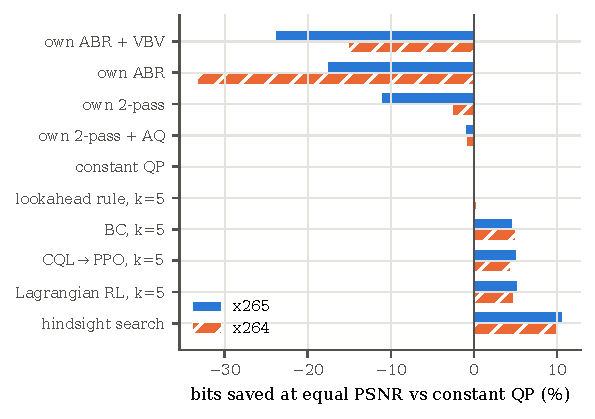
\includegraphics[width=\columnwidth]{figs/ownrc.pdf}
\caption{Bits saved at equal PSNR relative to the encoder's own constant QP (test). The encoders' built-in rate control falls below constant QP on 30-frame budgets; learned single-pass policies save 4.5--5.2\%; the hindsight search saves $\sim$10\%.}
\label{fig:ownrc}
\end{figure}

\subsection{How much does each frame of lookahead buy?}\label{sec:lookahead}
Fig.~\ref{fig:lookahead} shows the score of \cqlppo{} as a function of $k$, with the hand-designed lookahead rule, the constrained policies and the ceiling. Fig.~\ref{fig:share} and Table~\ref{tab:share} give the share of the search's saving.

\begin{figure*}[t]
\centering
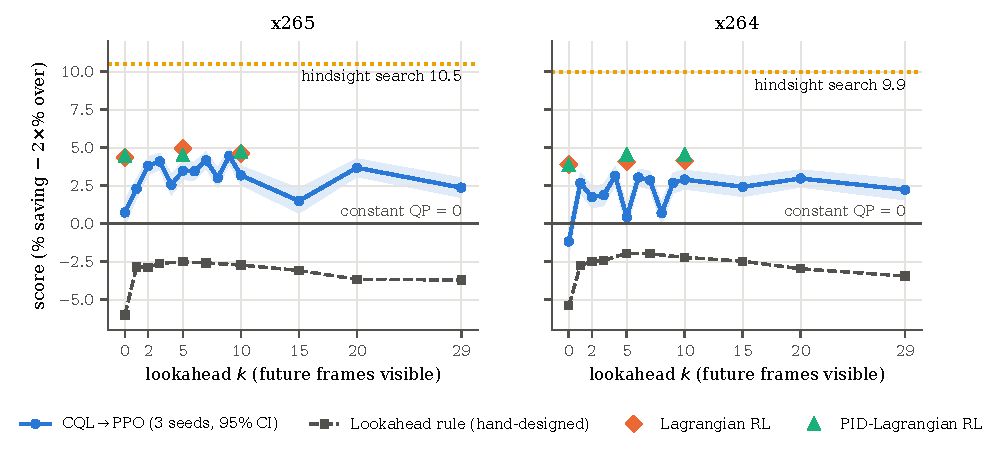
\includegraphics[width=0.9\textwidth]{figs/lookahead_score.pdf}
\caption{Score versus lookahead $k$ (test, 958 cases; band: 95\% CI). Learned policies are far above the hand-designed lookahead rule at every $k$. The gain is concentrated in the first 2--3 frames; beyond that the curve is flat within seed noise, and the full GOP ($k{=}29$) is not better than $k{=}2$. Budget-constrained RL (diamonds, triangles) is the best single-pass controller at every $k$ tested.}
\label{fig:lookahead}
\end{figure*}

\begin{figure}[t]
\centering
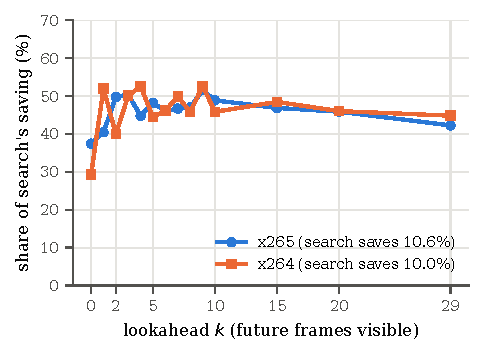
\includegraphics[width=0.9\columnwidth]{figs/share_vs_k.pdf}
\caption{Share of the hindsight search's bit saving captured by the single-pass \cqlppo{} policy. About half of the saving is recovered from $k{=}2$ on; additional frames do not increase the share.}
\label{fig:share}
\end{figure}

\begin{table}[t]
\centering\footnotesize
\caption{\cqlppo{} versus lookahead (test). Saving (\%) and share of the search's saving; score and share of the search's score.}
\label{tab:share}
\setlength{\tabcolsep}{3.5pt}
\begin{tabular}{@{}r cc cc | cc@{}}
\toprule
 & \multicolumn{4}{c|}{x265} & \multicolumn{2}{c}{x264}\\
$k$ & saving & share & score & share & saving & share\\
\midrule
0 & 3.97 & 37\% & 0.74 & 7\% & 2.94 & 29\%\\
1 & 4.29 & 40\% & 2.30 & 22\% & 5.21 & 52\%\\
2 & 5.28 & 50\% & 3.81 & 36\% & 4.01 & 40\%\\
3 & 5.34 & 50\% & 4.10 & 39\% & 5.03 & 50\%\\
5 & 5.11 & 48\% & 3.48 & 33\% & 4.45 & 44\%\\
7 & 4.95 & 47\% & 4.17 & 40\% & 5.00 & 50\%\\
10 & 5.18 & 49\% & 3.18 & 30\% & 4.60 & 46\%\\
20 & 4.87 & 46\% & 3.68 & 35\% & 4.62 & 46\%\\
29 & 4.48 & 42\% & 2.37 & 22\% & 4.50 & 45\%\\
\midrule
search & 10.61 & 100\% & 10.53 & 100\% & 10.03 & 100\%\\
\bottomrule
\end{tabular}
\end{table}

Three findings stand out. (i) \emph{The first frames are what counts.} On x265, going from $k{=}0$ to $k{=}1$ adds $+1.56\pm0.43$ score points and from 1 to 2 another $+1.51\pm0.30$, i.e., about 15 percentage points of the search's score per frame; on x264, $k{=}0\to1$ adds $+3.85\pm0.56$. (ii) \emph{Beyond 2--3 frames the curve is flat.} Neighbouring values of $k$ differ by up to $\pm1.5$ points, the same size as the differences between seeds, and the saving share stays at 46--52\% from $k{=}2$ to $k{=}20$ on x265. (iii) \emph{The whole GOP is not better.} At $k{=}29$ the saving is below that at $k{=}2$--9 on x265: a longer window adds inputs without information the policy can exploit. For a live encoder, a 2--3-frame lookahead buffer captures essentially all of the lookahead benefit that a single-pass policy can use at this GOP length; the remaining half of the search's gain is not a matter of seeing further, since the search observes actual encode outcomes that a policy must predict.

The learned policies are far above the hand-designed lookahead rule given the same information (+6 to +8 points at every $k$), so the gain comes from learning how to use the lookahead, not from the lookahead alone. By GOP type (x265, $k{=}5$), the policy's saving advantage over the rule is largest for GOPs with strong hard cuts (+9.6 points) and moderate cuts (+8.0), and smallest for low-motion GOPs without cuts (+3.7).

\subsection{Which learning approach?}\label{sec:methods}
Table~\ref{tab:methods} compares eleven approaches at $k{=}0$ and $k{=}5$.

\begin{table*}[t]
\centering\footnotesize
\caption{Learning approaches (test, 958 cases, 3 seeds averaged per case). Score / saving (\%) / share of cases $>$1\% over budget. Best score per column in bold.}
\label{tab:methods}
\begin{tabular}{@{}l l cccc@{}}
\toprule
Family & Method & x265, $k{=}0$ & x265, $k{=}5$ & x264, $k{=}0$ & x264, $k{=}5$\\
\midrule
\multirow{3}{*}{Imitation / offline} & BC & 1.68 / 3.68 / 17\% & 3.77 / 4.58 / 9\% & 0.21 / 3.12 / 19\% & 2.65 / 4.98 / 21\%\\
 & CQL & $-3.42$ / 2.51 / 29\% & $-1.77$ / 3.25 / 26\% & $-4.07$ / 2.24 / 29\% & $-1.23$ / 3.37 / 25\%\\
 & IQL & 2.04 / 3.49 / 10\% & $-0.63$ / 3.44 / 23\% & $-2.48$ / 2.58 / 25\% & 0.35 / 3.50 / 18\%\\
\midrule
\multirow{2}{*}{Offline$\to$online} & \bcppo & 2.80 / 4.05 / 10\% & 3.17 / 4.86 / 14\% & 2.46 / 3.59 / 8\% & 3.60 / 4.69 / 10\%\\
 & \cqlppo & 0.74 / 3.97 / 22\% & 3.48 / 5.11 / 15\% & $-1.17$ / 2.94 / 25\% & 0.43 / 4.45 / 24\%\\
\midrule
\multirow{3}{*}{Online, scratch} & PPO & 0.41 / 2.05 / 10\% & 0.32 / 2.13 / 14\% & $-0.74$ / 1.35 / 15\% & 0.15 / 1.80 / 14\%\\
 & A2C & 0.53 / 0.97 / 3\% & $-0.47$ / 0.62 / 8\% & 1.04 / 1.15 / 1\% & $-0.04$ / 1.18 / 7\%\\
 & DQN & 0.27 / 1.54 / 8\% & $-1.41$ / 0.20 / 11\% & 0.53 / 0.96 / 3\% & $-0.23$ / 0.96 / 6\%\\
\midrule
\multirow{2}{*}{Constrained RL} & Lagrangian & 4.36 / 4.63 / 1\% & \textbf{4.95} / 5.22 / 2\% & \textbf{3.90} / 4.22 / 2\% & 4.07 / 4.79 / 6\%\\
 & PID-Lagrangian & \textbf{4.46} / 5.00 / 4\% & 4.48 / 4.96 / 4\% & 3.83 / 4.29 / 4\% & \textbf{4.53} / 5.16 / 6\%\\
\midrule
Model-based & MPC (CEM) & $-1.78$ / $-0.72$ / 6\% & $-0.43$ / 0.70 / 7\% & $-3.58$ / $-0.54$ / 10\% & $-2.46$ / 0.56 / 10\%\\
\bottomrule
\end{tabular}
\end{table*}

\textbf{Online RL from scratch fails within this sample budget.} PPO, A2C and DQN save only 0.2--2.1\%. With 2{,}000 episodes, each requiring 30 real encodes, there is too little experience to learn a 346-dimensional policy from a terminal reward. A2C and DQN are conservative (few overshoots) because they barely leave the STATIC pattern.

\textbf{Imitation provides most of the saving.} BC on the search's best plans saves 3.7--5.0\%, close to \cqlppo{}. PPO fine-tuning raises the saving by about 0.5 points at $k{=}5$ (\cqlppo{} vs.\ BC on x265: $+0.53$ [+0.21, +0.83]) but also raises overshoot, so its score is not higher.

\textbf{Pure offline RL underperforms imitation here.} CQL and IQL trained on all logged plans overshoot more than BC: the logged dataset is dominated by search proposals near STATIC, and the conservative penalty keeps the policy close to that distribution.

\textbf{MPC exploits its model.} The learned bit model is unbiased on average (median actual/predicted GOP bits 1.03), yet CEM selects plans the model underestimates. Planning against a reduced budget helps, but every run chose the most conservative margin offered (0.6), and MPC stays below constant QP in saving. The planner's objective, not the model's accuracy, is the bottleneck.

\subsection{Where RL helps (1): budget reliability}
Constrained RL is the best single-pass controller in every column of Table~\ref{tab:methods}. Fig.~\ref{fig:constraint} and Table~\ref{tab:constraint} isolate its effect against imitation. At $k{=}0$, Lagrangian RL beats BC by +2.68 [+2.21, +3.15] points on x265 and +3.68 [+3.05, +4.35] on x264, and reduces the share of over-budget cases by 15.7 and 17.2 percentage points, \emph{while also saving more bits} (+0.95 and +1.10). The advantage shrinks as lookahead grows (x265: +1.19 at $k{=}5$, +0.37 at $k{=}10$), because a policy that sees ahead can anticipate expensive frames on its own. Imitation copies the search's plan; constrained RL makes the plan hold the budget in closed loop, which matters most when the controller cannot see what is coming.

\begin{figure*}[t]
\centering
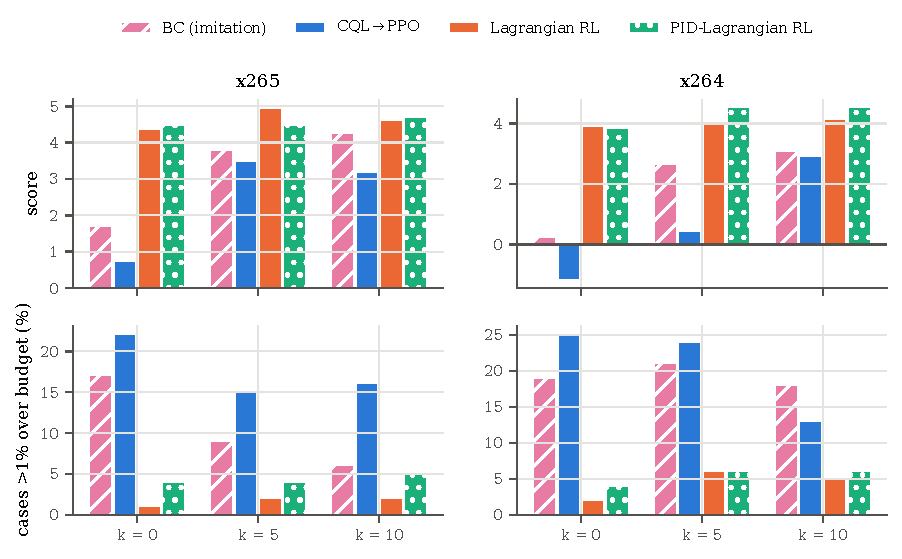
\includegraphics[width=0.85\textwidth]{figs/constraint.pdf}
\caption{Imitation versus RL in the per-GOP setting. Top: score; bottom: share of cases more than 1\% over budget. Constrained RL (Lagrangian, PID) is better than imitation (BC) and than unconstrained \cqlppo{}, and keeps 1--6\% of cases over budget versus 6--25\%.}
\label{fig:constraint}
\end{figure*}

\begin{table}[t]
\centering\footnotesize
\caption{Constrained RL minus BC (paired, 95\% bootstrap CI). Over: change in the share of cases $>$1\% over budget, percentage points.}
\label{tab:constraint}
\setlength{\tabcolsep}{2.5pt}
\begin{tabular}{@{}llccc@{}}
\toprule
 & $k$ & score & saving & over (pp)\\
\midrule
\multirow{3}{*}{x265, Lagr.} & 0 & +2.68 [2.21, 3.15] & +0.95 [0.64, 1.27] & $-15.7$\\
 & 5 & +1.19 [0.77, 1.64] & +0.64 [0.24, 1.03] & $-6.7$\\
 & 10 & +0.37 [0.01, 0.73] & +0.07 [$-$0.24, 0.40] & $-4.8$\\
\midrule
\multirow{3}{*}{x264, Lagr.} & 0 & +3.68 [3.05, 4.35] & +1.10 [0.72, 1.47] & $-17.2$\\
 & 5 & +1.42 [0.94, 1.90] & $-0.19$ [$-$0.48, 0.09] & $-14.5$\\
 & 10 & +1.06 [0.58, 1.53] & $-0.33$ [$-$0.62, $-$0.03] & $-12.4$\\
\midrule
\multirow{3}{*}{x264, PID} & 0 & +3.62 [3.01, 4.26] & +1.17 [0.81, 1.53] & $-15.7$\\
 & 5 & +1.88 [1.42, 2.34] & +0.18 [$-$0.10, 0.46] & $-15.1$\\
 & 10 & +1.45 [0.97, 1.93] & +0.17 [$-$0.09, 0.41] & $-12.0$\\
\bottomrule
\end{tabular}
\end{table}

\subsection{Where RL helps (2): budgets shared across GOPs}\label{sec:multigop}
Table~\ref{tab:multigop} and Fig.~\ref{fig:multigop} report the multi-GOP setting of Section~\ref{sec:mgdef}. The hand rule, which spends the remaining budget evenly over the remaining GOPs, loses heavily without lookahead ($-20.7$ on x265, $-44.9$ on x264) because it cannot know whether the first GOP is cheap or expensive. Imitation of the hindsight plan barely improves on it ($-17$ to $-20$): the plan's per-GOP QPs are optimal given every GOP's true rate--distortion curve, and copying them without that information produces systematic misallocation. RL, trained on the true objective with the policy's own information, learns to hedge: \bcppo{} with 2 GOPs of lookahead reaches $+3.23$ [+2.79, +3.64] on x265 and $+1.86$ [+1.34, +2.36] on x264, \emph{above the best constant QP chosen in hindsight}, with 1\% of cases over budget. PPO from scratch matches \bcppo{} with 2-GOP lookahead, since this environment is cheap enough for 2M training steps. Lookahead of two GOPs is worth +1.6 to +1.8 points over none. The three seeds agree closely (x265 \bcppo, $L{=}2$: 3.17, 3.24, 3.27). Relative to the best constant QP, the single-pass policy captures 26\% (x265) and 15\% (x264) of the hindsight plan's gain.

\begin{table}[t]
\centering\footnotesize
\caption{Multi-GOP streams (8 GOPs, one budget; test, 912 cases). Score / share of cases $>$1\% over budget. $L$: GOPs of lookahead. CI: 95\% bootstrap over cases.}
\label{tab:multigop}
\setlength{\tabcolsep}{3pt}
\begin{tabular}{@{}lcc@{}}
\toprule
Method & x265 & x264\\
\midrule
Hand rule, $L{=}0$ & $-20.68$ / 27\% & $-44.86$ / 33\%\\
Hand rule, $L{=}2$ & $-10.37$ / 27\% & $-14.08$ / 34\%\\
BC (imitation), $L{=}0$ & $-16.99$ / 10\% & $-16.06$ / 9\%\\
BC (imitation), $L{=}2$ & $-19.56$ / 7\% & $-19.63$ / 7\%\\
Best constant QP (hindsight) & 0 / 0\% & 0 / 0\%\\
PPO, $L{=}0$ & 0.96 / 2\% & $-0.77$ / 2\%\\
PPO, $L{=}2$ & 3.04 / 1\% & 1.87 / 1\%\\
\bcppo, $L{=}0$ & 1.65 / 1\% & 0.11 / 2\%\\
\bcppo, $L{=}2$ & \textbf{3.23} / 1\% & \textbf{1.86} / 1\%\\
\quad CI vs.\ constant QP & [+2.79, +3.64] & [+1.34, +2.36]\\
Hindsight per-GOP plan & 12.54 / 0\% & 12.45 / 0\%\\
\bottomrule
\end{tabular}
\end{table}

\begin{figure}[t]
\centering
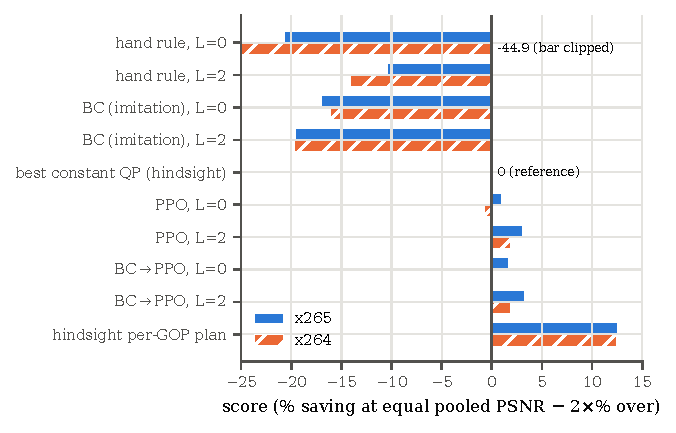
\includegraphics[width=\columnwidth]{figs/multigop.pdf}
\caption{Multi-GOP streams. Imitating the hindsight plan fails without its information; RL policies are the only causal controllers above the best constant QP chosen in hindsight.}
\label{fig:multigop}
\end{figure}

\subsection{Extensions and ablations}
Table~\ref{tab:ext} summarizes further variants at $k{=}5$. A 3-seed ensemble of \cqlppo{} raises the x265 score by +1.04 [+0.73, +1.38] and the saving by +0.53; on x264 it raises the score from 0.43 to 3.44. Lagrangian and PID fine-tuning of the finished \cqlppo{} policy lowers overshoot to 5--6\% at a small cost in saving. Feedback features (achieved PSNR, bit-prediction error) do not help; window-summary features are neutral at $k{=}5$ and help at $k{=}29$, consistent with long raw windows being hard to use. Warm-started A2C collapses towards STATIC (saving 1.8\%, 0\% over), and warm-started DQN does not retain the CQL initialization. A per-frame gate between the $k{=}0$ and $k{=}5$ policies does not beat always using $k{=}5$; the learned gate's usage of lookahead varied from 20\% to 98\% across seeds. Removing feature groups shows that first-pass costs are the most important input (x265 score 3.48 $\to$ $-0.97$ without them), followed by pixel statistics and history, while scene flags are redundant given first-pass costs. Scene-aware lookahead (truncating the window at the next cut) and a single any-$k$ network perform on par with fixed $k{=}5$ (x265: 3.91 and 4.50).

\begin{table}[t]
\centering\footnotesize
\caption{Extensions at $k{=}5$ (test). Score / saving (\%) / share $>$1\% over.}
\label{tab:ext}
\setlength{\tabcolsep}{2.5pt}
\begin{tabular}{@{}lcc@{}}
\toprule
Variant & x265 & x264\\
\midrule
\cqlppo{} (reference) & 3.48 / 5.11 / 15\% & 0.43 / 4.45 / 24\%\\
3-seed ensemble & \textbf{4.52} / \textbf{5.63} / 11\% & 3.44 / \textbf{5.58} / 14\%\\
+ Lagrangian fine-tune & 4.10 / 4.74 / 6\% & \textbf{4.13} / 4.78 / 5\%\\
+ PID fine-tune & 4.03 / 4.64 / 5\% & 3.17 / 4.63 / 10\%\\
Feedback features & 2.72 / 4.88 / 18\% & 2.50 / 4.98 / 21\%\\
Summary features & 3.40 / 4.59 / 13\% & 3.44 / 4.60 / 9\%\\
Summary features, $k{=}29$ & 3.68 / 4.93 / 9\% & 3.93 / 4.95 / 7\%\\
Gate $k{=}0/k{=}5$, $\lambda{=}1$ & 3.17 / 4.76 / 14\% & 1.09 / 4.29 / 20\%\\
CQL$\to$A2C & 1.79 / 1.82 / 0\% & 1.48 / 1.86 / 3\%\\
CQL$\to$DQN & $-1.72$ / 0.69 / 14\% & $-1.72$ / 0.79 / 14\%\\
No first-pass features & $-0.97$ / 3.07 / 24\% & $-1.07$ / 3.67 / 27\%\\
No scene features & 3.40 / 4.59 / 10\% & 3.23 / 5.27 / 15\%\\
\bottomrule
\end{tabular}
\end{table}

%=====================================================================
\section{Discussion}\label{sec:discussion}
%=====================================================================
\textbf{When to expect RL to beat imitation.} Our results fit a simple rule. When the expert's actions are good choices \emph{given the learner's information}, imitation captures most of the value with far fewer samples than RL, as in per-frame control within a GOP, where the search's decisions depend mostly on visible frame costs. When the expert's actions depend on information the learner lacks, here the future GOPs' rate--distortion curves and the exact QP that meets a stream budget, imitation reproduces actions out of context and fails, while RL optimizes for the information it actually has. Constraints are a second case: the expert never faces the learner's prediction errors, so only training in closed loop teaches a policy to absorb them, which is what constrained RL does.

\textbf{Sample cost, not RL itself, limited RL here.} Online RL from scratch failed when each episode cost 30 real encodes, but PPO from scratch matched imitation-initialized PPO in the multi-GOP environment, where 2M steps were affordable. Cheaper simulators of the encoder are therefore the main lever for RL in rate control. Our first attempt at a learned simulator (PPO trained inside the MPC bit/PSNR model, then fine-tuned on real encodes) showed the policy's in-model score rising far faster than its real score could, the signature of model exploitation, and diverged when model PSNR left the range of the real constant-QP curve. Anchoring the model to each GOP's real STATIC encode and bounding its PSNR change are in place; results are pending.

\textbf{Metric choices matter.} Averaging PSNR in dB across GOPs rewards spending bits on cheap static GOPs; with that average, a hindsight plan reached a 36\% ``saving'' in the multi-GOP setting. Pooling MSE removes this artefact and is what we report. Similarly, the score rewards saving at equal PSNR at any operating point, so the hindsight multi-GOP plan often runs below budget; this does not change the ranking of causal controllers but should be kept in mind when reading its absolute value.

\textbf{Agreement with an independent replication.} An independent pipeline (different preset, 208 test GOPs, clipped saving) found the same shape of the lookahead curve, the same ordering of the encoders' rate-control modes, small effects of gating and scene features, and the same reliability-for-saving trade of constrained RL. Absolute savings differ by about $2.4\times$, and it found the ensemble and warm-started A2C to behave differently, so these two results should be treated as setup-dependent.

\textbf{Threats to validity.} Results are for $320{\times}180$ video, 30-frame IDR GOPs without B frames, and with AQ and CU-/MB-tree disabled for controlled encodes; the encoders' own rate control was evaluated on the same short budgets, which disadvantages controllers designed for long streams. Quality is PSNR only. The multi-GOP setting controls one QP per GOP and reads outcomes from real constant-QP encodes, so it does not include frame-level control. Seed variance at a single $k$ ($\pm$1.5 points) is comparable to the differences between adjacent $k$; only the overall shape of the lookahead curve, not individual points beyond $k{=}3$, is supported. We did not measure policy inference latency.

%=====================================================================
\section{Future Work}
%=====================================================================
\begin{itemize}
\item \textbf{Model-based pre-training.} Complete the anchored model-based experiment and compare real-encode sample efficiency with \cqlppo; add uncertainty-aware rollouts (ensembles, short horizons~\cite{janner2019mbpo}).
\item \textbf{Hierarchical control.} Combine the multi-GOP budget policy with the per-frame policy, so that GOP-level allocation and frame-level allocation are learned jointly.
\item \textbf{Objectives the search did not optimize.} Perceptual quality (SSIM~\cite{wang2004ssim}, VMAF~\cite{li2016vmaf}), quality-fluctuation penalties and per-frame size caps, where imitation of a PSNR-optimal teacher is mis-targeted by construction.
\item \textbf{Realistic coding structures.} B frames, AQ and CU-tree enabled, longer GOPs, higher resolutions, and integration into the encoder's lookahead thread with measured latency.
\item \textbf{Fairer encoder baselines} on long streams, and a qcomp-tuned variant of the encoders' own rate control.
\item \textbf{Calibrated MPC.} Re-weight the planner's PSNR-versus-overshoot objective, whose optimum lay at the edge of every margin grid we tried.
\end{itemize}

%=====================================================================
\section{Conclusion}
%=====================================================================
An offline search that sees a whole GOP saves about 10\% of the bits of constant QP at equal PSNR, on budgets where x264's and x265's own rate control fall below constant QP. A single-pass learned policy recovers about half of that saving, and two to three frames of lookahead are enough to reach it: for a live encoder at this GOP length, more delay does not buy more quality. Imitating the search is the most sample-efficient way to obtain the saving. Reinforcement learning earns its place where imitation cannot reach: it makes the policy reliable under its budget, with the largest gain when the controller cannot see ahead, and it is the only approach tested that beats the best constant QP when several GOPs share one budget whose matching QP is unknown.

\section*{Acknowledgment}
Computation was performed on the USC Center for Advanced Research Computing (CARC) cluster.

\begin{thebibliography}{99}\footnotesize
\bibitem{sullivan1998rdo} G. J. Sullivan and T. Wiegand, ``Rate-distortion optimization for video compression,'' \emph{IEEE Signal Process. Mag.}, vol.~15, no.~6, pp.~74--90, Nov. 1998.
\bibitem{ortega1998rd} A. Ortega and K. Ramchandran, ``Rate-distortion methods for image and video compression,'' \emph{IEEE Signal Process. Mag.}, vol.~15, no.~6, pp.~23--50, Nov. 1998.
\bibitem{garrett2009mbtree} J. Garrett-Glaser, ``A novel macroblock-tree algorithm for high-performance optimization of dependent video coding in H.264/AVC,'' Tech. Rep., 2009.
\bibitem{x264} VideoLAN, ``x264: a free H.264/AVC encoder.'' [Online]. Available: \url{https://www.videolan.org/developers/x264.html}
\bibitem{x265} MulticoreWare, ``x265 HEVC encoder documentation.'' [Online]. Available: \url{https://x265.readthedocs.io}
\bibitem{wiegand2003h264} T. Wiegand, G. J. Sullivan, G. Bj{\o}ntegaard, and A. Luthra, ``Overview of the H.264/AVC video coding standard,'' \emph{IEEE Trans. Circuits Syst. Video Technol.}, vol.~13, no.~7, pp.~560--576, Jul. 2003.
\bibitem{sullivan2012hevc} G. J. Sullivan, J.-R. Ohm, W.-J. Han, and T. Wiegand, ``Overview of the High Efficiency Video Coding (HEVC) standard,'' \emph{IEEE Trans. Circuits Syst. Video Technol.}, vol.~22, no.~12, pp.~1649--1668, Dec. 2012.
\bibitem{chen2007rcsurvey} Z. Chen and K. N. Ngan, ``Recent advances in rate control for video coding,'' \emph{Signal Process.: Image Commun.}, vol.~22, no.~1, pp.~19--38, 2007.
\bibitem{li2014lambda} B. Li, H. Li, L. Li, and J. Zhang, ``$\lambda$ domain rate control algorithm for High Efficiency Video Coding,'' \emph{IEEE Trans. Image Process.}, vol.~23, no.~9, pp.~3841--3854, Sep. 2014.
\bibitem{bjontegaard2001} G. Bj{\o}ntegaard, ``Calculation of average PSNR differences between RD-curves,'' ITU-T SG16 Q.6, Doc. VCEG-M33, Austin, TX, Apr. 2001.
\bibitem{sutton2018rl} R. S. Sutton and A. G. Barto, \emph{Reinforcement Learning: An Introduction}, 2nd ed. Cambridge, MA: MIT Press, 2018.
\bibitem{williams1992reinforce} R. J. Williams, ``Simple statistical gradient-following algorithms for connectionist reinforcement learning,'' \emph{Mach. Learn.}, vol.~8, pp.~229--256, 1992.
\bibitem{konda2000actorcritic} V. R. Konda and J. N. Tsitsiklis, ``Actor-critic algorithms,'' in \emph{Proc. NeurIPS}, 2000.
\bibitem{mnih2016a3c} V. Mnih \emph{et al.}, ``Asynchronous methods for deep reinforcement learning,'' in \emph{Proc. ICML}, 2016.
\bibitem{schulman2017ppo} J. Schulman, F. Wolski, P. Dhariwal, A. Radford, and O. Klimov, ``Proximal policy optimization algorithms,'' arXiv:1707.06347, 2017.
\bibitem{schulman2016gae} J. Schulman, P. Moritz, S. Levine, M. Jordan, and P. Abbeel, ``High-dimensional continuous control using generalized advantage estimation,'' in \emph{Proc. ICLR}, 2016.
\bibitem{mnih2015dqn} V. Mnih \emph{et al.}, ``Human-level control through deep reinforcement learning,'' \emph{Nature}, vol.~518, pp.~529--533, 2015.
\bibitem{pomerleau1989alvinn} D. A. Pomerleau, ``ALVINN: An autonomous land vehicle in a neural network,'' in \emph{Proc. NeurIPS}, 1989.
\bibitem{ross2011dagger} S. Ross, G. Gordon, and D. Bagnell, ``A reduction of imitation learning and structured prediction to no-regret online learning,'' in \emph{Proc. AISTATS}, 2011.
\bibitem{levine2020offline} S. Levine, A. Kumar, G. Tucker, and J. Fu, ``Offline reinforcement learning: Tutorial, review, and perspectives on open problems,'' arXiv:2005.01643, 2020.
\bibitem{kumar2020cql} A. Kumar, A. Zhou, G. Tucker, and S. Levine, ``Conservative Q-learning for offline reinforcement learning,'' in \emph{Proc. NeurIPS}, 2020.
\bibitem{kostrikov2022iql} I. Kostrikov, A. Nair, and S. Levine, ``Offline reinforcement learning with implicit Q-learning,'' in \emph{Proc. ICLR}, 2022.
\bibitem{altman1999cmdp} E. Altman, \emph{Constrained Markov Decision Processes}. Boca Raton, FL: Chapman \& Hall/CRC, 1999.
\bibitem{tessler2019rcpo} C. Tessler, D. J. Mankowitz, and S. Mannor, ``Reward constrained policy optimization,'' in \emph{Proc. ICLR}, 2019.
\bibitem{stooke2020pid} A. Stooke, J. Achiam, and P. Abbeel, ``Responsive safety in reinforcement learning by PID Lagrangian methods,'' in \emph{Proc. ICML}, 2020.
\bibitem{rubinstein1997cem} R. Y. Rubinstein, ``Optimization of computer simulation models with rare events,'' \emph{Eur. J. Oper. Res.}, vol.~99, no.~1, pp.~89--112, 1997.
\bibitem{chua2018pets} K. Chua, R. Calandra, R. McAllister, and S. Levine, ``Deep reinforcement learning in a handful of trials using probabilistic dynamics models,'' in \emph{Proc. NeurIPS}, 2018.
\bibitem{sutton1991dyna} R. S. Sutton, ``Dyna, an integrated architecture for learning, planning, and reacting,'' \emph{ACM SIGART Bull.}, vol.~2, no.~4, pp.~160--163, 1991.
\bibitem{janner2019mbpo} M. Janner, J. Fu, M. Zhang, and S. Levine, ``When to trust your model: Model-based policy optimization,'' in \emph{Proc. NeurIPS}, 2019.
\bibitem{lakshminarayanan2017ensembles} B. Lakshminarayanan, A. Pritzel, and C. Blundell, ``Simple and scalable predictive uncertainty estimation using deep ensembles,'' in \emph{Proc. NeurIPS}, 2017.
\bibitem{hu2018rlintra} J.-H. Hu, W.-H. Peng, and C.-H. Chung, ``Reinforcement learning for HEVC/H.265 intra-frame rate control,'' in \emph{Proc. IEEE ISCAS}, 2018.
\bibitem{schrittwieser2020muzero} J. Schrittwieser \emph{et al.}, ``Mastering Atari, Go, chess and shogi by planning with a learned model,'' \emph{Nature}, vol.~588, pp.~604--609, 2020.
\bibitem{mandhane2022muzero} A. Mandhane \emph{et al.}, ``MuZero with self-competition for rate control in VP9 video compression,'' arXiv:2202.06626, 2022.
\bibitem{wang2019ugc} Y. Wang, S. Inguva, and B. Adsumilli, ``YouTube UGC dataset for video compression research,'' in \emph{Proc. IEEE MMSP}, 2019.
\bibitem{xiph} Xiph.Org Foundation, ``Xiph.org video test media (derf's collection).'' [Online]. Available: \url{https://media.xiph.org/video/derf/}
\bibitem{blender} Blender Foundation, ``Open movies: Big Buck Bunny, Elephants Dream, Sintel, Tears of Steel.'' [Online]. Available: \url{https://studio.blender.org/films/}
\bibitem{raffin2021sb3} A. Raffin, A. Hill, A. Gleave, A. Kanervisto, M. Ernestus, and N. Dormann, ``Stable-Baselines3: Reliable reinforcement learning implementations,'' \emph{J. Mach. Learn. Res.}, vol.~22, no.~268, pp.~1--8, 2021.
\bibitem{towers2024gymnasium} M. Towers \emph{et al.}, ``Gymnasium: A standard interface for reinforcement learning environments,'' arXiv:2407.17032, 2024.
\bibitem{efron1993bootstrap} B. Efron and R. J. Tibshirani, \emph{An Introduction to the Bootstrap}. New York: Chapman \& Hall, 1993.
\bibitem{wang2004ssim} Z. Wang, A. C. Bovik, H. R. Sheikh, and E. P. Simoncelli, ``Image quality assessment: From error visibility to structural similarity,'' \emph{IEEE Trans. Image Process.}, vol.~13, no.~4, pp.~600--612, Apr. 2004.
\bibitem{li2016vmaf} Z. Li, A. Aaron, I. Katsavounidis, A. Moorthy, and M. Manohara, ``Toward a practical perceptual video quality metric,'' Netflix Technology Blog, Jun. 2016.
\end{thebibliography}

\end{document}
